\documentclass[11.5pt, paper=a4]{article}

\usepackage[utf8]{inputenc}
\usepackage[english]{babel}
\usepackage[T1]{fontenc}

\usepackage{amsmath, amssymb, amscd, amsthm, amsfonts, mathtools}
\usepackage[left=2cm, right=2cm, top=1.5cm]{geometry}

\usepackage{graphicx}
\usepackage{hyperref}
\usepackage{physics}
\usepackage{tikz}
\usepackage{url}
\usepackage[square,numbers]{natbib}
\usepackage{tabularx}

\usepackage{braket}
\usepackage{thmtools}
\usepackage{float}

%%% Theorem Style
\theoremstyle{definition}
\newtheorem{theorem}{Theorem}[section]
\newtheorem{definition}[theorem]{Definition}
\newtheorem{lemma}[theorem]{Lemma}
\newtheorem{conjecture}[theorem]{Conjecture}
\newtheorem{corollary}[theorem]{Corollary}

\numberwithin{theorem}{section}

%% Autoref prefixes
\renewcommand{\sectionautorefname}{Section}
\renewcommand{\subsectionautorefname}{Section}
\renewcommand{\subsubsectionautorefname}{Section}
\renewcommand{\figureautorefname}{Figure}
\def\theoremautorefname{Theorem}
\def\lemmaautorefname{Lemma}
\def\definitionautorefname{Definition}
\def\conjectureautorefname{Conjecture}
\def\algorithmautorefname{Algorithm}

%% Writing algorithms

\usepackage{algorithm} % captioning 
\usepackage{algpseudocode}
\usepackage{multirow}
\usepackage{qcircuit}

% \def\NoNumber#1{{\def\alglinenumber##1{}\State #1}\addtocounter{ALG@line}{-1}}

\graphicspath{{./Lecture_5/images/}}


\title{Quantum Algorithms, Spring 2022: Lecture 5 Scribe}

\author{Praguna Manvi, Samay Kathari}

\date{\today}

\begin{document}

\maketitle

\section{Recap}

\begin{itemize}
    \item Reversible circuits produce unwanted garbage bits that are dependent on the input and are entangle with the desired out bits, so we need : \textbf{Uncomputing!}
    \begin{equation*}
        \Qcircuit @C=1em @R=.7em {
            & \lstick{\ket{x}} & \multigate{1}{C_f} & \qw & \rstick{\ket{x}} \\
            & \lstick{\ket{y}} & \ghost{C_f} & \qw & \rstick{\ket{y \bigoplus f(x)}} \\
        }
    \end{equation*}
    \item Quantum Circuits
    \begin{itemize}
        \item Single Qubit Gates: $X, Y, Z, R_\phi, h, \ldots$
        \item Two Qubit Gates: CNOT, any $C-U$ where U is a single qubit gate.
        \begin{equation*}
            \Qcircuit @C=1em @R=.7em {
            & \lstick{\ket{c}} & \ctrl{1} & \qw & \rstick{\ket{e}} \\
            & \lstick{\ket{t}} & \gate{U} & \qw & \rstick{U^c\ket{t}} \\
        }
        \end{equation*}
        \begin{equation*} 
            \equiv
            \begin{pmatrix}
                1 & 0 & 1 & 0\\
                0 & 1 & 0 & 1\\
                0 & 0 & \multicolumn{2}{c}{\multirow{2}{*}{U}}\\
                0 & 0 &
            \end{pmatrix}
        \end{equation*}
        $\forall$ U is any single qubit gate.
    \end{itemize}
\end{itemize}

\section{Universality of Quantum circuits}

I will provide you some statements regarding the universality of quantum circuits without necessarily proving them.
\begin{itemize}
    \item \textbf{Statement 1:} \{CNOT, all single qubit gates\} : universal for Quantum Computing
    \item \textbf{Statement 2:} The set of \{ CNOT, $H$, $R_{\pi/4}\}$ : universal for Quantum Computing \\
    \textit{Any other quantum circuit can be well approximated using quantum circuits of only these gates.}
\end{itemize}
\subsection{Formalizing Statement 2}
    Let $G=\{CNOT, H, R_{\pi/4}\}$, then for any quantum circuit $U$, $\in$ a number $t$, such that
    \begin{equation*}
        \lvert\lvert U - U_t U_{t-1} \ldots U_1 \rvert\rvert \leq \epsilon, where
    \end{equation*}
    \begin{center}
        each $U_j \in G$ \\ $\lvert \lvert \quad \rvert \rvert:$ spectral norm \\ $\lvert \lvert A \rvert \rvert = max_{\bra{\psi}\ket{\psi}=1} \lvert \lvert A\ket{\psi} \rvert \rvert$
    \end{center}
    \begin{itemize}
        \item How large should 't' be? Clearly, it better not be too large.
        \item Luckily 't' isn't too large owing to crucial result by Solvay and Kitaev
    \end{itemize}
\section{Solovay Ketanov Theorem}
\begin{itemize}
    \item Any 't'-gate quantum circuit can be $\epsilon$ approximated using only $\mathcal{O}(t$ polylog$ (\frac{1}{\epsilon}))$ gates from G.
    \item \textbf{Proof:} Appendix of Neilsen and Chuang \cite{nielsen2002quantum}
    \item There are also other universal gate sets: some are efficient than others.
\end{itemize}

\section{Quantum Parallelism}

\begin{itemize}
    \item Suppose we are interested in some function $f:\{0,1\}^n\xrightarrow{}\{0,1\}$
    \begin{equation*}
        \Qcircuit @C=1em @R=.7em {
            & \lstick{\ket{x}} & \multigate{1}{U_f} & \qw & \rstick{\ket{x}} \\
            & \lstick{\ket{y}} & \ghost{U_f} & \qw & \rstick{\ket{y \bigoplus f(x)}} \\
        }
    \end{equation*}
    So, if $f(x)=0$, \quad $\ket{x}\ket{y}\xrightarrow{U_f}\ket{x}\ket{y}$ \\
    and if $f(x)=1$, \quad $\ket{x}\ket{y}\xrightarrow{U_f}\ket{x}\ket{\Bar{y}}$ \\
    \begin{equation*}
        \Qcircuit @C=1em @R=.7em {
            \lstick{\ket{0}} &\qw & \gate{H} & \multigate{3}{U_f} & \qw & \qw & \meter\\
            \lstick{\vdots} & \qw & \qw & \ghost{U_f} & \qw & \qw & \meter\\
            \lstick{\ket{0}} &\qw & \gate{H} & \ghost{U_f} & \qw & \qw & \meter \\
            \lstick{\ket{0}} &\qw & \qw & \ghost{U_f} & \qw & \qw
        }
    \end{equation*}
    \begin{equation*}
        \ket{0}^{\bigotimes n}\ket{0} \xrightarrow{H^{\bigotimes n}\mathbb{1}}\frac{1}{\sqrt{2^n}}\sum_{x\in\{0,1\}^n}\ket{x}\ket{0}\xrightarrow{U_f}\frac{1}{\sqrt{2^n}}\sum_{x\in\{0,1\}^n}\ket{x}\ket{f(x)}
    \end{equation*}
    \item By applying $U_f$ only once, we are able to obtain a quantum state that contains in it all $2^n$ possible values of $f(x)$ in superposition!
    \item This in itself is not very useful. If we make projective measurement, we will observe some $\ket{z}\ket{f(z)}$ with probability $1/2^n$.
    \item Quantum parallelism is not enough to demonstrate the power of quantum computing.
    \item Quantum parallelism needs to be combined with interference, entanglement, to something better than classical computing. 
\end{itemize}



\section{Quantum Oracle : Phase Kickback Oracle}
\begin{itemize}
    \item From the above sections we know that for some function : 
    $f : \{0, 1\}^n \xrightarrow{}\{0,1\}$ and \\ 
    \begin{equation*}
            \Qcircuit @C=1em @R=.7em {
                & \lstick{\ket{x}} & \multigate{1}{U_f} & \qw & \rstick{\ket{x}} \\
                & \lstick{\ket{y}} & \ghost{U_f} & \qw & \rstick{\ket{y \bigoplus f(x)}} \\
            }
    \end{equation*}
    \begin{equation*}
        \text{if\quad} f(x)=0, \text{\quad} \ket{x}\ket{y}\xrightarrow{U_f}\ket{x}\ket{y}
    \end{equation*}
    \begin{equation*}
        \text{and if\quad} f(x)=1, \text{\quad} \ket{x}\ket{y}\xrightarrow{U_f}\ket{x}\ket{\Bar{y}}
    \end{equation*}
    If we substitute $\ket{-}$ for $y$ we get :
        \begin{equation*}
        \text{if\quad} f(x)=0, \text{\quad} \ket{x}[\frac{\ket{0} - \ket{1}}{\sqrt{2}}]\xrightarrow{U_f}\ket{x}[\frac{\ket{0} - \ket{1}}{\sqrt{2}}]
    \end{equation*}
    \begin{equation*}
        \text{and if\quad} f(x)=1, \text{\quad} \ket{x}[\frac{\ket{0} - \ket{1}}{\sqrt{2}}]\xrightarrow{U_f}-\ket{x}[\frac{\ket{0} - \ket{1}}{\sqrt{2}}]
    \end{equation*}
\item The phase get changed when $f(x) = 1$ (a kickback), hence we call this a phase kick back oracle with whose result we can guess $f(x)$ !
This can be rewritten as :
\begin{equation*}
    \ket{x}\ket{-} \xrightarrow{U_f} (-1)^{f(x)}\ket{x}\ket{-}
\end{equation*}
Rewriting the circuit for $y = \ket{-}$:
\begin{equation*}
     \Qcircuit @C=1em @R=.7em {
                & \lstick{\ket{x}} & \multigate{1}{U_f} & \qw & \qw & \rstick{(-1)^{f(x)}\ket{x}} \\
                \lstick{\ket{1}} & \gate{H} & \ghost{U_f} & \qw & \qw & \rstick{\ket{-}} \\
        }
\end{equation*}
The second input and output lines can be dropped as they remain the same in another frequently used representation :
\begin{equation*}
     \Qcircuit @C=1em @R=.7em {
                & \lstick{\ket{x}} & \gate{U_f^{\pm}} & \qw & \qw & \rstick{(-1)^{f(x)}\ket{x}}\\
        }
\end{equation*}
\begin{equation*}
    \ket{x} \xrightarrow{U_f^{\pm}} (-1)^{f(x)}\ket{x}
\end{equation*}
On passing $H^{\bigotimes n}\ket{0^{\bigotimes n}}$ into the phase kickback $U_f^{\pm}$ we get :
\begin{equation*}
    H^{\bigotimes n}\ket{0^{\bigotimes n}} 
    \xrightarrow{U_f^{\pm}} \frac{1}{\sqrt{2^n}} \sum_{x\in\{0,1\}^n} \ket{x}
    \xrightarrow{U_f^{\pm}} \frac{1}{\sqrt{2^n}} \sum_{x\in\{0,1\}^n} (-1)^{f(x)}\ket{x}
\end{equation*}
The important thing to note here is that after passing through the oracle the amplitudes of the states have the information of $f(x)$
\end{itemize}

\section{Deutsch Algorithm}
Given a $U_f$ for some boolean function $f : \{0, 1\} \xrightarrow{} \{0, 1\}$ with the promise that either : $f(0) = f(1)$ or $f(0) \neq
f(1) $, the task is to find the number of queries to $U_f$ to determine which is the case.
\begin{itemize}
  \item Classical Algorithm requires 2 queries by comparing outputs of inputs 0 and 1.
  \item Quantum Algorithm requires only 1 query! with the design :
    \begin{equation*}
            \Qcircuit @C=1em @R=.7em {
              \lstick{\ket{0}} & \gate{H} & \gate{U_f^{\pm}} & \gate{H} & \meter
            }
    \end{equation*}
\begin{equation*}
    H\ket{0} = \frac{1}{\sqrt{2}}({\ket{0} + \ket{1}}) \xrightarrow{U_f^{\pm}}\ \frac{1}{\sqrt{2}}({-1^{f(0)}\ket{0} + -1^{f(1)}\ket{1}})\xrightarrow{H}\frac{(-1^{f(0)} + -1^{f(1)})\ket{0} + (-1^{f(0)} - 1^{f(1)})\ket{1}}{2}
\end{equation*}
we observe : 
\begin{equation*}
    \ket{0} \text{\:if\:} f(0) = f(1), and\:
    \ket{1} \text{\:for\:} f(0) \neq f(1)
\end{equation*}
Therefore, only one query with input $\ket{0}$ is needed.
\end{itemize}

\section{Physics Understanding of the Deutsch Problem}

The physical setup of the Deutsch Algorithm is realised using Mach Zehnder Interferometer which consists of a beam splitter that creates an equal superposition of $\ket{0}$ and $\ket{1}$. The phase shifter adds a phase of $0$ or $\pi$ which passes through another beam splitter (acting as final $H$ gate in Deutsch Algorithm) where the final states are recorded. 

\begin{figure}[H]
    \centering
    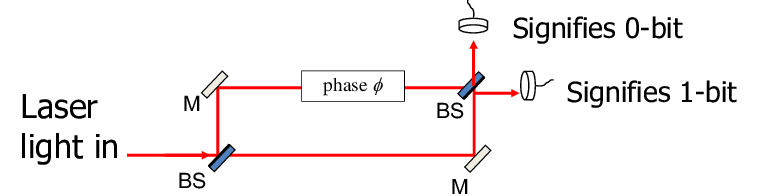
\includegraphics[scale=0.5]{mz.png}\\
    \caption{mach zehnder interferometer [2]}
    \label{fig : mach zehnder interferometer}
\end{figure}



\nocite{*}
\bibliographystyle{plainnat}
\bibliography{references}

\end{document}
